\documentclass{article}
\usepackage[margin=1in]{geometry}
\usepackage{graphicx, chngcntr, multirow, float, subcaption, pgfplots}
\usepackage[labelfont=bf,textfont=md]{caption}

\pgfplotsset{width=.99\textwidth,compat=1.9}

\counterwithin{figure}{section}

\title{CS-521 Term Project: Packet vs. Circuit Switching}
\author{Lucas Ferreira, Vishal Rao, Justin Ho}
\date{29 April 2021}

\begin{document}
  \maketitle

  {\flushleft We pledge our honor that we have abided by the Stevens Honor System.

  \textit{Lucas Ferreira, Vishal Rao, Justin Ho}}

  \section{Introduction}

  Packet-switched networks break streams of data into small blocks known as packets. Each of these packets are then sent
  independently over a shared network, based on the destination address in each packet. After receiving, packets are reassembled
  in the proper sequence to make up the message. Data is processed at all intermediate node including source system. The
  delay between data units is not uniform. It is suitable for handling bilateral traffic. And, multiple users can use the
  same channel while transferring their packets. If one route is failed the data can be routed from other paths too.

  Circuit-switched networks require dedicated point-to-point connections. The resources needed are reserved for the duration
  of the communication between the end systems. It was designed specifically for voice communication and packet switched
  networks handled data. Data is processed only at source system. And, the delay between data units is uniform. Circuit
  switching is not convenient for handling bilateral traffic. It is preferred when the communication is long and continuous.

  To compare the performance of packet-switched and circuit-switched networks, we created an event-based simulation model
  for either network. A series of experiments were designed to test how either network reacts to packets being sent across
  them, and whether one has an overall better performance than the other.


  \section{Analysis}

  \subsection{Methodology}

  To compare and contrast the performance of packet switching and circuit switching, two event-based simulation models
  written in Python were created to simulate a packet switching network and a circuit switching network. The intent of
  creating these models was to provide numerical insight into how the time data packets spend traveling through a network
  is affected by the effects of packet switching and circuit switching. By generating statistics such as average data packet
  queue delay and average data packet total delay for a network simulation, a strong basis for comparing the two types of
  networks was formulated.

  For both simulations, a simple bi-directional network graph consisting of six nodes was used, as shown in Figure 2.1, where fixed-size data packets
  are randomly generated at node 0, and sent through the network where their destination is always node 5. The models
  created allow for the mean arrival rate of each new data packet, the total simulation duration, and the transmission time
  between nodes to be manually set. For example, a circuit switching simulation could be run with a new packet mean arrival time of 500 milliseconds, a
  total simulation duration of two hours, and a transmission time between nodes of 80 milliseconds. Note that the transmission delay
  at the network nodes is disregarded. At the end of each simulation, the results, which include average queue delay and total delay statistics, are printed to the console.

  \begin{figure}[h]
  \centering
          \includegraphics[totalheight=6cm]{images/network_graph.png}
  \renewcommand\figurename{Figure}
      \caption{Network graph used in simulation model}
      \label{fig:networkgraph}
  \end{figure}

  The circuit switching model simulates the way circuit switching networks are implemented by dedicating an entire channel
  through the network from source to destination when a data packet is ready to be transmitted. Whenever new data packets are generated and cannot be transmitted
  because the there are no available channels, they enter a queue where they remain until new channels become available. This
  process is illustrated in Figure 2.2. The packet switching model has a different mechanism for handling channels when data packets
  are being transmitted through the network. Rather than securing the entire channel from a data packet's destination node to its
  source node, the packet switching model only secures individual channels between two different nodes as a data packet moves throughout its
  assigned path. For example, if a data packet being transmitted from node 0 to node 5, which has been assigned the path 0-1-2-5, is
  traveling through the 1-2 channel, only the 1-2 channel is secured, and thus blocked. Whenever a data packet arrives at a new node,
  it checks if the next channel it needs to use is available. If it isn't, it searches for a new channel which can lead the data packet
  to its destination. If no other channels are available, the data packet is inserted into a queue belonging to the last node it
  visited. As new channels become available, the data packet is popped from the queue and resumes its trip to its destination. The
  packet switching process is illustrated in Figure 2.3.

  \begin{figure}[h]
    \centering
    \includegraphics[totalheight=5.5cm]{images/graph_cs.png}
    \renewcommand\figurename{Figure}
    \caption{Circuit switching model}
    \label{fig:graph_cs}
  \end{figure}

  \begin{figure}[H]
    \centering
    \includegraphics[totalheight=8cm]{images/graph_ps.png}
    \renewcommand\figurename{Figure}
    \caption{Packet switching model}
    \label{fig:graph_ps}
  \end{figure}
  
  \subsection{Graphs and Tables}

  All time measurements are in milliseconds.

  \begin{table}[h!]
    \caption{Circuit Switching Simulation Results}
    \centering
    {\footnotesize
      \begin{tabular}{|c|c|c|c|c|c|}
        \hline
        Transmit Time & Avg. Arrival Time & Packets Arrived & Packets Completed & Avg. Total Delay
        & Avg. Queue Delay\\  
        \hline

        \multirow{5}{*}{20} & 42 & 85,825 & 85,821 & 43.36 & 0.3\\
        \cline{2-6}
        & 54 & 66,553 & 66,551 & 42.17 & 0.12\\
        \cline{2-6}
        & 66 & 54,428 & 54,426 & 41.48 & 0.06\\
        \cline{2-6}
        & 78 & 46,126 & 46,125 & 41.09 & 0.03\\
        \cline{2-6}
        & 90 & 39,815 & 39,814 & 40.8 & 0.02\\
        \hline

        \multirow{5}{*}{30} & 42 & 85,668 & 85,666 & 70.03 & 2.14\\
        \cline{2-6}
        & 54 & 67,008 & 67,006 & 66.56 & 0.77\\
        \cline{2-6}
        & 66 & 54,354 & 54,352 & 64.55 & 0.33\\
        \cline{2-6}
        & 78 & 46,304 & 46,303 & 63.51 & 0.2\\
        \cline{2-6}
        & 90 & 40,209 & 40,207 & 62.68 & 0.11\\
        \hline

        \multirow{5}{*}{40} & 42 & 85,680 & 85,678 & 105.92 & 12.0\\
        \cline{2-6}
        & 54 & 66,557 & 66,553 & 94.26 & 3.31\\
        \cline{2-6}
        & 66 & 54,436 & 54,435 & 89.94 & 1.51\\
        \cline{2-6}
        & 78 & 46,193 & 46,191 & 87.49 & 0.71\\
        \cline{2-6}
        & 90 & 40,027 & 40,026 & 85.85 & 0.42\\
        \hline

        \multirow{5}{*}{50} & 42 & 85,511 & 85,509 & 232.07 & 112.28\\
        \cline{2-6}
        & 54 & 66,922 & 66,919 & 130.07 & 13.05\\
        \cline{2-6}
        & 66 & 54,719 & 54,715 & 118.76 & 4.78\\
        \cline{2-6}
        & 78 & 46,151 & 46,149 & 113.65 & 2.21\\
        \cline{2-6}
        & 90 & 39,984 & 39,983 & 110.78 & 1.27\\
        \hline
      \end{tabular}
    }
  \end{table}

  \begin{table}[h!]
    \caption{Packet Switching Simulation Results}
    \centering
    {\footnotesize
      \begin{tabular}{|c|c|c|c|c|c|}
        \hline
        Transmit Time & Avg. Arrival Time & Packets Arrived & Packets Completed & Avg. Total Delay
        & Avg. Queue Delay\\
        \hline

        \multirow{5}{*}{20} & 42 & 85,627 & 85,625 & 40.72 & 0.03\\
        \cline{2-6}
        & 54 & 66,748 & 66,746 & 40.42 & 0.01\\
        \cline{2-6}
        & 66 & 54,707 & 54,705 & 40.28 & 0.01\\
        \cline{2-6}
        & 78 & 46,332 & 46,331 & 40.18 & 0.01\\
        \cline{2-6}
        & 90 & 39,849 & 39,848 & 40.15 & 0.01\\
        \hline

        \multirow{5}{*}{30} & 42 & 85,741 & 85,739 & 62.96 & 0.21\\
        \cline{2-6}
        & 54 & 66,621 & 66,619 & 61.6 & 0.09\\
        \cline{2-6}
        & 66 & 54,514 & 54,513 & 61.01 & 0.04\\
        \cline{2-6}
        & 78 & 46,247 & 46,245 & 60.71 & 0.02\\
        \cline{2-6}
        & 90 & 39,977 & 39,975 & 60.49 & 0.01\\
        \hline

        \multirow{5}{*}{40} & 42 & 85,516 & 85,512 & 88.75 & 0.82\\
        \cline{2-6}
        & 54 & 66,675 & 66,673 & 84.29 & 0.33\\
        \cline{2-6}
        & 66 & 54,294 & 54,291 & 82.57 & 0.14\\
        \cline{2-6}
        & 78 & 46,128 & 46,126 & 81.75 & 0.08\\
        \cline{2-6}
        & 90 & 39,969 & 39,966 & 81.23 & 0.04\\
        \hline

        \multirow{5}{*}{50} & 42 & 85,858 & 85,855 & 119.24 & 2.05\\
        \cline{2-6}
        & 54 & 66,559 & 66,555 & 110.16 & 0.95\\
        \cline{2-6}
        & 66 & 54,308 & 54,306 & 105.6 & 0.42\\
        \cline{2-6}
        & 78 & 46,172 & 46,170 & 103.77 & 0.23\\
        \cline{2-6}
        & 90 & 40,030 & 40,029 & 102.65 & 0.12\\
        \hline
      \end{tabular}
    }
  \end{table}

  \begin{figure}[h!]
    \caption{Circuit Switching vs. Packet Switching -- Avg. Arrival Time}
    \centering
    \begin{subfigure}{.5\textwidth}
      \centering
      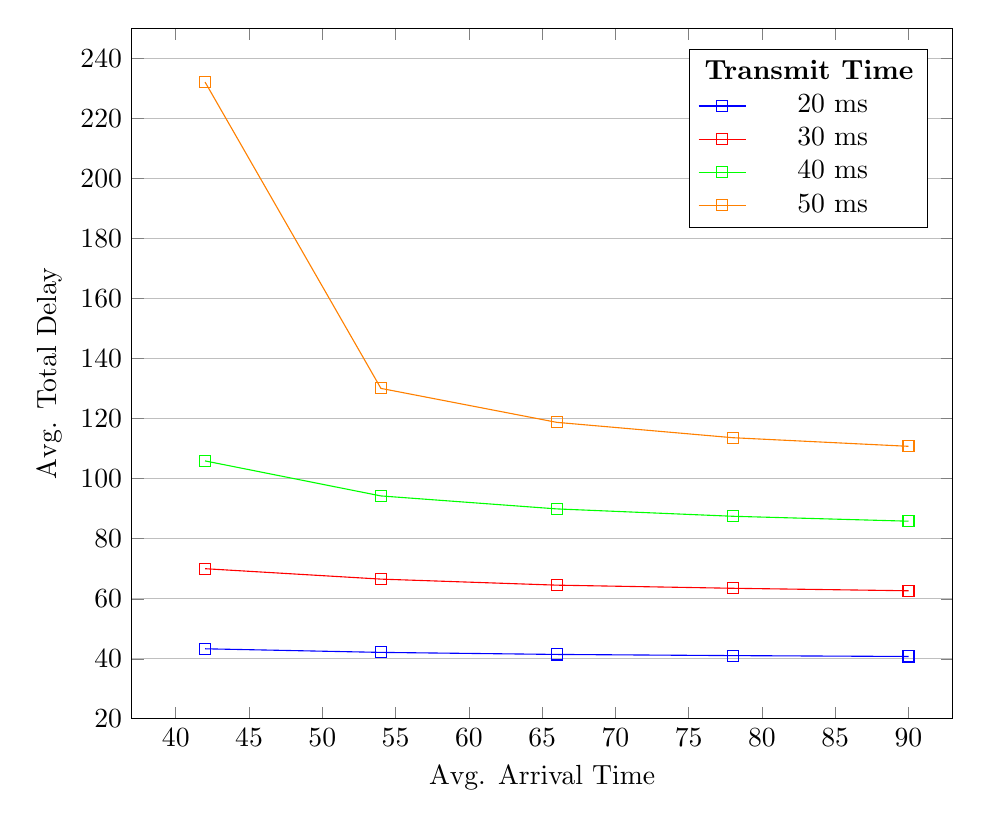
\begin{tikzpicture}
        \begin{axis}[
          xlabel={Avg. Arrival Time},
          ylabel={Avg. Total Delay},
          xmin=37, xmax=93,
          ymin=20, ymax=250,
          ymajorgrids=true,
          legend pos=north east
        ]
          \addlegendimage{empty legend}
          \addlegendentry{\hspace{-.6cm}\textbf{Transmit Time}}
          
          \addplot[
            color=blue,
            mark=square,
          ]
          coordinates {
            (42,43.36) (54,42.16) (66,41.48) (78,41.09) (90,40.8)
          };
          \addlegendentry{20 ms}

          \addplot[
            color=red,
            mark=square,
          ]
          coordinates {
            (42,70.03) (54,66.56) (66,64.55) (78,63.51) (90,62.68)
          };
          \addlegendentry{30 ms}

          \addplot[
            color=green,
            mark=square,
          ]
          coordinates {
            (42,105.92) (54,94.26) (66,89.94) (78,87.49) (90,85.85)
          };
          \addlegendentry{40 ms}

          \addplot[
            color=orange,
            mark=square,
          ]
          coordinates {
            (42,232.07) (54,130.07) (66,118.76) (78,113.65) (90,110.78)
          };
          \addlegendentry{50 ms}
        \end{axis}
      \end{tikzpicture}
      \caption{Circuit Switching}
    \end{subfigure}%
    \begin{subfigure}{.5\textwidth}
      \centering
      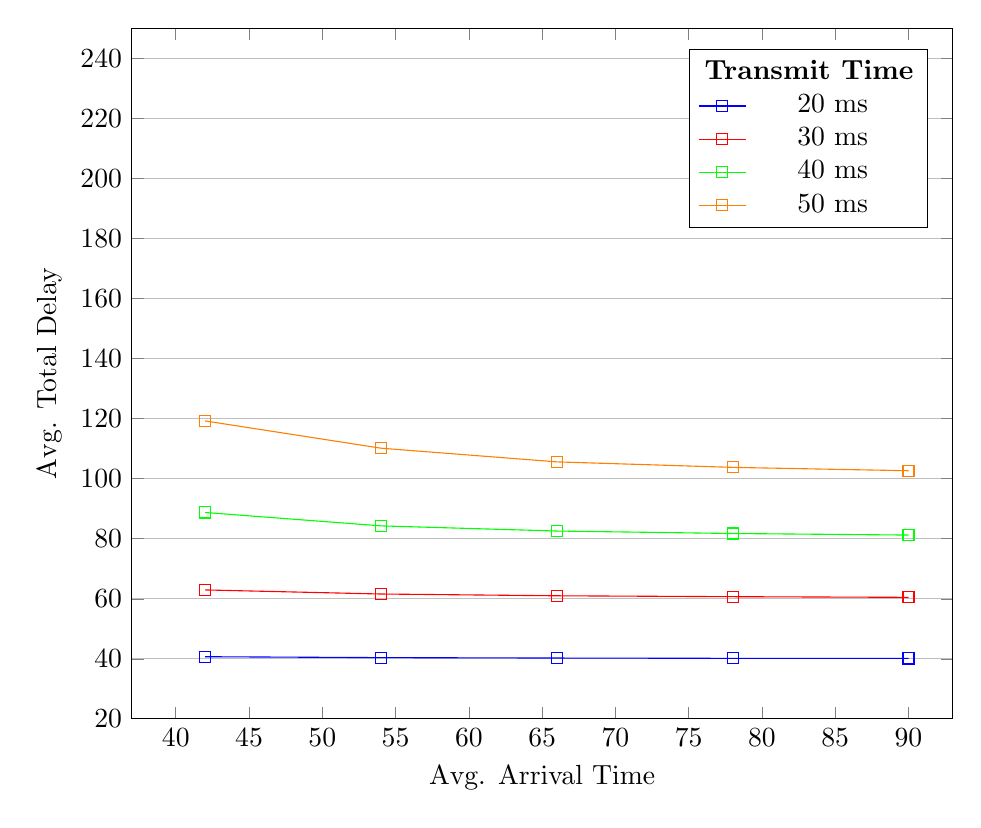
\begin{tikzpicture}
        \begin{axis}[
          xlabel={Avg. Arrival Time},
          ylabel={Avg. Total Delay},
          xmin=37, xmax=93,
          ymin=20, ymax=250,
          ymajorgrids=true,
          legend pos=north east
        ]
          \addlegendimage{empty legend}
          \addlegendentry{\hspace{-.6cm}\textbf{Transmit Time}}
          
          \addplot[
            color=blue,
            mark=square,
          ]
          coordinates {
            (42,40.72) (54,40.42) (66,40.28) (78,40.18) (90,40.15)
          };
          \addlegendentry{20 ms}

          \addplot[
            color=red,
            mark=square,
          ]
          coordinates {
            (42,62.96) (54,61.6) (66,61.01) (78,60.71) (90,60.49)
          };
          \addlegendentry{30 ms}

          \addplot[
            color=green,
            mark=square,
          ]
          coordinates {
            (42,88.75) (54,84.29) (66,82.57) (78,81.75) (90,81.23)
          };
          \addlegendentry{40 ms}

          \addplot[
            color=orange,
            mark=square,
          ]
          coordinates {
            (42,119.24) (54,110.16) (66,105.6) (78,103.77) (90,102.65)
          };
          \addlegendentry{50 ms}
        \end{axis}
      \end{tikzpicture}
      \caption{Packet Switching}
    \end{subfigure}
  \end{figure}

  \begin{figure}[h!]
    \caption{Circuit Switching vs. Packet Switching -- Transmission Time}
    \centering
    \begin{subfigure}{.5\textwidth}
      \centering
      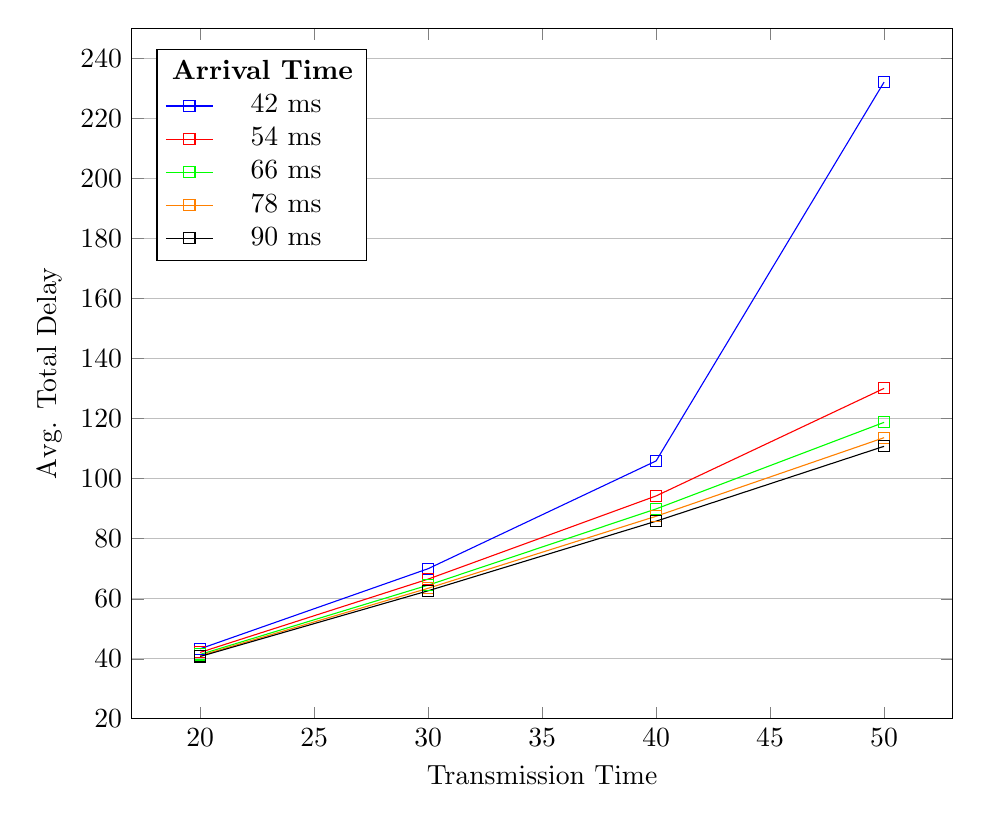
\begin{tikzpicture}
        \begin{axis}[
          xlabel={Transmission Time},
          ylabel={Avg. Total Delay},
          xmin=17, xmax=53,
          ymin=20, ymax=250,
          ymajorgrids=true,
          legend pos=north west
        ]
          \addlegendimage{empty legend}
          \addlegendentry{\hspace{-.6cm}\textbf{Arrival Time}}
          
          \addplot[
            color=blue,
            mark=square,
          ]
          coordinates {
            (20,43.36) (30,70.03) (40,105.92) (50,232.07)
          };
          \addlegendentry{42 ms}

          \addplot[
            color=red,
            mark=square,
          ]
          coordinates {
            (20,42.17) (30,66.56) (40,94.26) (50,130.07)
          };
          \addlegendentry{54 ms}

          \addplot[
            color=green,
            mark=square,
          ]
          coordinates {
            (20,41.48) (30,64.55) (40,89.94) (50,118.76)
          };
          \addlegendentry{66 ms}

          \addplot[
            color=orange,
            mark=square,
          ]
          coordinates {
            (20,41.09) (30,63.51) (40,87.49) (50,113.65)
          };
          \addlegendentry{78 ms}

          \addplot[
            color=black,
            mark=square,
          ]
          coordinates {
            (20,40.8) (30,62.68) (40,85.85) (50,110.78)
          };
          \addlegendentry{90 ms}
        \end{axis}
      \end{tikzpicture}
      \caption{Circuit Switching}
    \end{subfigure}%
    \begin{subfigure}{.5\textwidth}
      \centering
      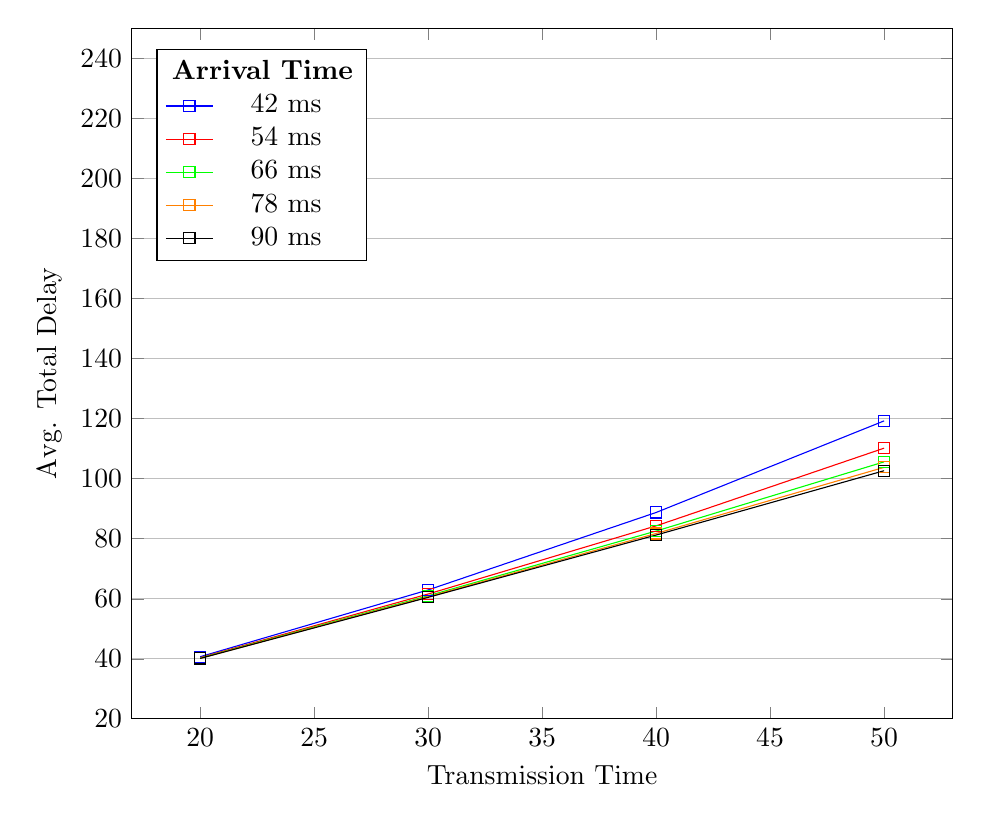
\begin{tikzpicture}
        \begin{axis}[
          xlabel={Transmission Time},
          ylabel={Avg. Total Delay},
          xmin=17, xmax=53,
          ymin=20, ymax=250,
          ymajorgrids=true,
          legend pos=north west
        ]
          \addlegendimage{empty legend}
          \addlegendentry{\hspace{-.6cm}\textbf{Arrival Time}}
          
          \addplot[
            color=blue,
            mark=square,
          ]
          coordinates {
            (20,40.72) (30,62.96) (40,88.75) (50,119.24)
          };
          \addlegendentry{42 ms}

          \addplot[
            color=red,
            mark=square,
          ]
          coordinates {
            (20,40.42) (30,61.6) (40,84.29) (50,110.16)
          };
          \addlegendentry{54 ms}

          \addplot[
            color=green,
            mark=square,
          ]
          coordinates {
            (20,40.28) (30,61.01) (40,82.57) (50,105.6)
          };
          \addlegendentry{66 ms}

          \addplot[
            color=orange,
            mark=square,
          ]
          coordinates {
            (20,40.18) (30,60.71) (40,81.75) (50,103.77)
          };
          \addlegendentry{78 ms}

          \addplot[
            color=black,
            mark=square,
          ]
          coordinates {
            (20,40.15) (30,60.49) (40,81.23) (50,102.65)
          };
          \addlegendentry{90 ms}
        \end{axis}
      \end{tikzpicture}
      \caption{Packet Switching}
    \end{subfigure}
  \end{figure}

  \section{Observations and Recommendations}



  \section{Conclusion}
\end{document}
